% This is slides.tex.
\documentclass[pdf]{beamer}
\mode<presentation>{}                % change the theme here

\usepackage{colortbl}
\usepackage{amsfonts}
\usepackage{amsmath}
\usepackage{amssymb}
\usepackage{amsthm}
\usepackage{graphicx}
\usepackage[dvipsnames]{xcolor}
\usepackage{url}
\usepackage{tikz}
\usetikzlibrary{shapes.geometric, arrows.meta, positioning}



\usepackage[backend=biber,style=numeric,sorting=none]{biblatex}
\usepackage{subcaption}
\setbeamertemplate{caption}[numbered]

%Change colors of your slides here. For list of named colors, see
% https://www.overleaf.com/learn/latex/Using_colors_in_LaTeX#Accessing_additional_named_colors

\usetheme{Madrid}
%this affects the color of your title text, and also the right color bar on the bottom
    \setbeamercolor{palette primary}{fg=white, bg = purple} 
%This is the middle color bar on the bottom of the slide
    \setbeamercolor{palette secondary}{bg=black!80,fg=white} 
%this is the left color bar on the bottom of the slide, along with the text there. !20 changes shade (lighter vs darker) 
    \setbeamercolor{palette tertiary}{bg=purple,fg=white!80} 
%unclear what this does... it might not be in use right now
    \setbeamercolor{palette quaternary}{bg=red!20,fg=black!80} 
% itemize, enumerate, and theorem headings
    \setbeamercolor{structure}{fg=purple!80} 
% examaple block
    \setbeamercolor{block title example}{bg = purple!50!black}
% table of contents
    \setbeamercolor{section in toc}{fg=red!20} 

% Override palette coloring with secondary
\setbeamercolor{subsection in head/foot}{bg=white,fg=white} 
\setbeamercolor{frametitle}{fg=white,bg=black!80}%this changes the header background and text color

% \addbibresource{biblio.bib}
\theoremstyle{plain}
\setbeamertemplate{navigation symbols}{} %comment this out if you want navigation tools on the slide
\setbeamertemplate{blocks}[rounded][shadow=false]

%be VERY careful editing this. If you do it wrong you'll break your slide
\title{GraphPeptideMiner}
\subtitle{A Knowledge-Layer Workflow for Extracting Peptide Self-Assembly Rules from Literature}
\author[David Shi]{David Shi\texorpdfstring{\\
Research Science Institute\\
Under the Direction of Prof. Markus J. Buehler \\
and Dr. Subhadeep Pal \\
Laboratory for Atomistic and Molecular Mechanics}{}} 
\date{July 9th, 2025}

\begin{document}

\begin{frame}
    \thispagestyle{empty}          % prevents page numbering on the title slide
    \titlepage
\end{frame}
\addtocounter{framenumber}{-1} % don't count title slide in the page numbering

\begin{frame}{Introduction}
    
    \begin{block}{Field of Study}
        \begin{itemize}
            \item Short-peptide self-assembly
            \item Variety of factors: sequence, concentration, pH, etc
            \item Existing benchmark: 1012 entries, 75 papers, \textasciitilde70\% accuracy
        \end{itemize}
    \end{block}

    \pause
    
    
    \begin{columns}
        \begin{column}{0.5\textwidth}
            \begin{block}{Research Gap}
                \begin{itemize}
                    \item Direct llm extraction is unreliable
                    \item Desired information is scattered
                    \vspace{0.1cm}
                \end{itemize}
            \end{block}{}
        \end{column}

        \hspace{0.1cm}
        \pause
        
        \begin{column}{0.4\textwidth}
            \begin{block}{Morphology}
                \centering
                
\includegraphics[width=0.8\textwidth]{"Modify/peptide rsi week 1 1.jpg"}
                {\tiny Source: de Groot et al., \textit{Biophys. J.}, 2007}
            \end{block}
        \end{column}
    \end{columns}

\end{frame}

\begin{frame}{Introduction}
    \begin{block}{Research Aim}
        \begin{itemize}
            \item Organize peptide papers into JSON records
            \item Validate records with RF / MLP 
            \item Package as reusable ScienceSkill
        \end{itemize}
    \end{block}

    \vspace{0.5cm}
    \pause
    
    \begin{columns}
        \begin{column}{0.4\textwidth}
            \begin{block}{Hypothesis}
                \begin{itemize}
                    \item \textbf{A graph-grounded multi-agent workflow improves extraction accuracy, traceability, and downstream phase prediction}
                \end{itemize}
            \end{block}
        \end{column}

        \hspace{0.1cm}
        \pause
        

        \begin{column}{0.5\textwidth}
            \begin{block}{Peptide Structure}
                \centering
                
\includegraphics[width=0.8\textwidth]{"Modify/rsi peptide week 1.jpg"}
                {\tiny Adler-Abramovich \& Gazit, \textit{J. Pept. Sci.}, 2008}
            \end{block}
        \end{column}

    \end{columns}

\end{frame}

\begin{frame}{Methods}
    \begin{block}{Workflow}
        \vspace{0.5cm}
        \begin{center}
        \resizebox{\textwidth}{!}{
        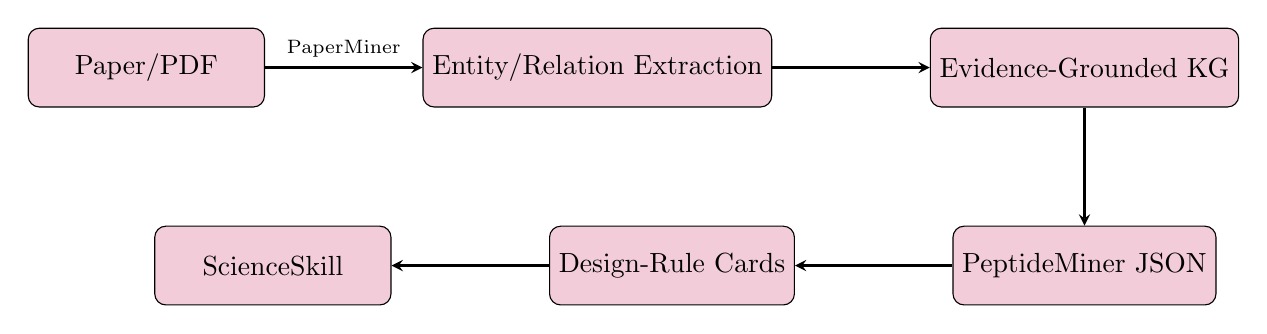
\begin{tikzpicture}[
            node distance=1.5cm and 2cm,
            process/.style={rectangle, minimum width=3cm, minimum height=1cm, text centered, draw=black, fill=purple!20, rounded corners},
            arrow/.style={thick,->,>=stealth}
            ]
            
            \node (pdf) [process] {Paper/PDF};
            \node (extract) [process, right=of pdf] {Entity/Relation Extraction};
            \node (kg) [process, right=of extract] {Evidence-Grounded KG};
            \node (json) [process, below=of kg] {PeptideMiner JSON};
            \node (rules) [process, left=of json] {Design-Rule Cards};
            \node (skill) [process, left=of rules] {ScienceSkill};
    
            \draw [arrow] (pdf) -- node[above, font=\scriptsize] {PaperMiner} (extract);
            \draw [arrow] (extract) -- (kg);
            \draw [arrow] (kg) -- (json);
            \draw [arrow] (json) -- (rules);
            \draw [arrow] (rules) -- (skill);
        \end{tikzpicture}
        }
        \end{center}
        \vspace{0.5cm}
        
    \end{block}
\end{frame}


\begin{frame}{Methods}
    \begin{block}{Data preparation}
        \begin{itemize}
            \item 75 paper benchmark
            \item Two stage document cleaning
            \item JSON schema extraction (GPT-5.5)
        \end{itemize}

    \end{block}

    \pause
    \vspace{1cm}

    \begin{block}{Validation}
        \begin{itemize}
            \item Graph path $\; \rightarrow \;$ JSON row
            \item Downstream phase prediction preservation
            \item Reusable ScienceSkill package prototype
        \end{itemize}
    \end{block}
\end{frame}

\begin{frame}{Methods}
    \begin{block}{Graph Schema}
        \begin{itemize}
            \item Link peptide \& exp. cond. to observed phase
            \item Multi-agent extraction:
            \begin{itemize} 
                \item Section, entity, relation, graph, verifier, table, and classifier agents.
            \end{itemize}
        \end{itemize}
    \end{block}

    \pause

    \begin{center}
        \begin{block}{Instantiated Graph Schema (Paper 1, Experiment 1)}
            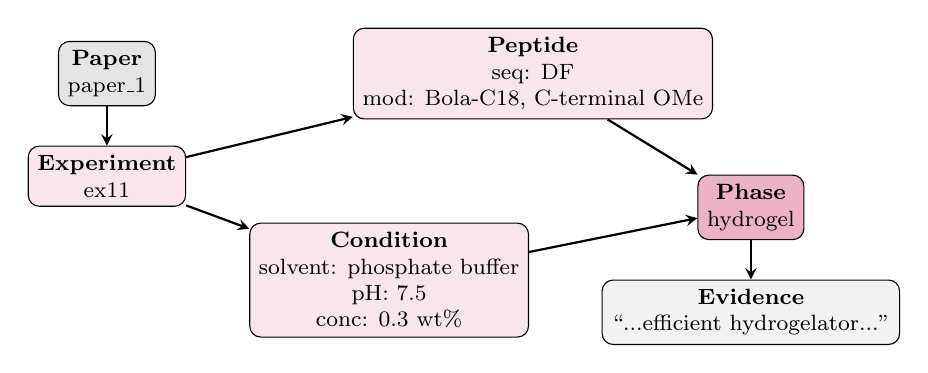
\begin{tikzpicture}[
                font=\footnotesize,
                node distance=0.5cm and 0.5cm,
                box/.style={rectangle, draw, rounded corners, align=center, fill=purple!10, minimum height=0.6cm},
                widebox/.style={box, text width=3.5cm},
                arrow/.style={thick,->,>=stealth}
            ]
            \node (paper) [box, fill=gray!20] {\textbf{Paper}\\paper\_1};
            \node (exp) [box, below= 0.5cm of paper] {\textbf{Experiment}\\ex11};
            
            \node (pep) [box, right=2.5cm of paper] {\textbf{Peptide}\\seq: DF\\mod: Bola-C18, C-terminal OMe};
            \node (cond) [box, below right =0.2cm and 0.8cm of exp] {\textbf{Condition}\\solvent: phosphate buffer\\pH: 7.5\\conc: 0.3 wt\%};
            \node (phase) [box, fill=purple!30, below right= 0.7cm and -0.2cm of pep] {\textbf{Phase}\\hydrogel};
            \node (evi) [box, fill=gray!10, below=0.5cm of phase] {\textbf{Evidence}\\``...efficient hydrogelator...''};
    
            \draw [arrow] (paper) -- (exp);
            \draw [arrow] (exp) -- (pep);
            \draw [arrow] (exp) -- (cond);
            \draw [arrow] (pep) -- (phase);
            \draw [arrow] (cond) -- (phase);
            \draw [arrow] (phase) -- (evi);
            \end{tikzpicture}
        \end{block}
    \end{center}
\end{frame}

\begin{frame}{Results}
    \begin{block}{Manual Benchmark}
        \begin{itemize}
            \item Human verified extraction logs
            \item Isolated relevant factors:
            \begin{itemize}
                \item Sequence, modifications, solvent, concentration, pH, temperature, and phase data
            \end{itemize}
        \end{itemize}
    \end{block}

    \pause
    \vspace{1cm}

    \begin{block}{Cleaning Pipeline}
        \begin{itemize}
            \item .pdf $\; \rightarrow \;$ .md conversion
            \item Standardized JSON records
        \end{itemize}
    \end{block}
    
\end{frame}

\begin{frame}{Acknowledgements}
\begin{itemize}
    \item Prof Markus J. Buehler - LAMM
    \item Dr. Subhadeep Pal - LAMM
    
\end{itemize}



\includegraphics[width=0.25\textwidth]{Modify/images/rsi.jpeg}

\includegraphics[width=0.4\textwidth]{Modify/images/mit.jpeg}
\raisebox{1\totalheight}{
\includegraphics[width=0.25\textwidth]{Modify/images/cee.jpeg}}
\end{frame}




\end{document}